\chapter{Results}
\cite{jon}
 
\section{Pion Spectra}

The efficiency correction is applied track-by-track, where the efficiency of the i-th track $\epsilon_i$ is retrieved from the database, from the parameters discussed in Section~\ref{sec:efficiency}. The correction factor $C_i$ is defined as,

\begin{equation}
C_i = \epsilon_i^{-1}.
\end{equation}

Each track that is identified as a pion, is then weighted by the correction factor $C_i$, when filling any histogram. By using the track-by-track method, we can transform the track into any observable of interest, notably we can transform the  track from the lab frame into the center-of-mass (CM) frame. Before performing the transformation to the CM system recall the beam is at a small, but non-negligible, angle in the Lab frame, see Section~\ref{sec:beamangle}. The beam angle for each even is measured and a rotation is applied to all the tracks in an event, to align the beam angle along the z-axis. Doing so makes the transformation into the CM system much simpler to describe. If the beam direction is defined by a unit vector $\hat{b}$, we can define the rotation that rotates the beam into the z-axis as a rotation about an arbitrary vector $\hat{v} = \hat{b}\times\hat{z}$ where the angle between the two is given by $\cos \theta = \hat{b}\cdot\hat{z}$. 

Once all the events have been rotated to align with the z-axis, transforming from the Lab to the CM frame is done by a Lorentz transformation. Where the 4-momentum vector in the lab frame is defined as $\textbf{P} = (E/c,p_x,p_y,p_z)$. Where the corresponding Lorentz transform into the CM frame along the beam (z-axis) is defined as,

\begin{equation}
A = \begin{pmatrix}
1 & 0 & 0 & 0\\
0 & 1 & 0 & 0\\
0 & 0 & \gamma & -\beta \gamma\\
0 & 0 & -\beta \gamma & \gamma
\end{pmatrix},
\end{equation}

where $\beta$, describes the velocity of the CM system, and $\gamma=\sqrt{1-\beta^2}^{-1}$. The parameter $\beta$ can be determined from the total momentum of the system in the Laboratory frame $P = \sqrt{ T_{P}^2 - M_{T}^2}$ and the total energy of the system $E = T_{P} + M_{P} + M_{T}$ as $\beta = -P/E$, where the (-) sign denotes the correct direction for transforming from the Lab to the CM frame. The CM transformed track is defined as $p^{CM} = \textbf{A}p^{Lab}$.


%need to add error analysis
%systematic error analysis


Figure~\ref{fig:pionspectra} shows the pion CM kinetic energy spectra for both the $\tin{132}{124}$ and $\tin{108}{112}$ systems. This data marks the first pion spectral data at sub-threshold energies, extending to very low pion energies. The coulomb potential works to accelerate $\pi^+$ and decelerate $\pi^-$ particles due to the positive charge of the nuclear medium. The coulomb barrier prevents the production of low energy $\pi^+$, which is why there is a reduction in the phase space around zero kinetic energy. 

\begin{figure}[!htb]
\centering
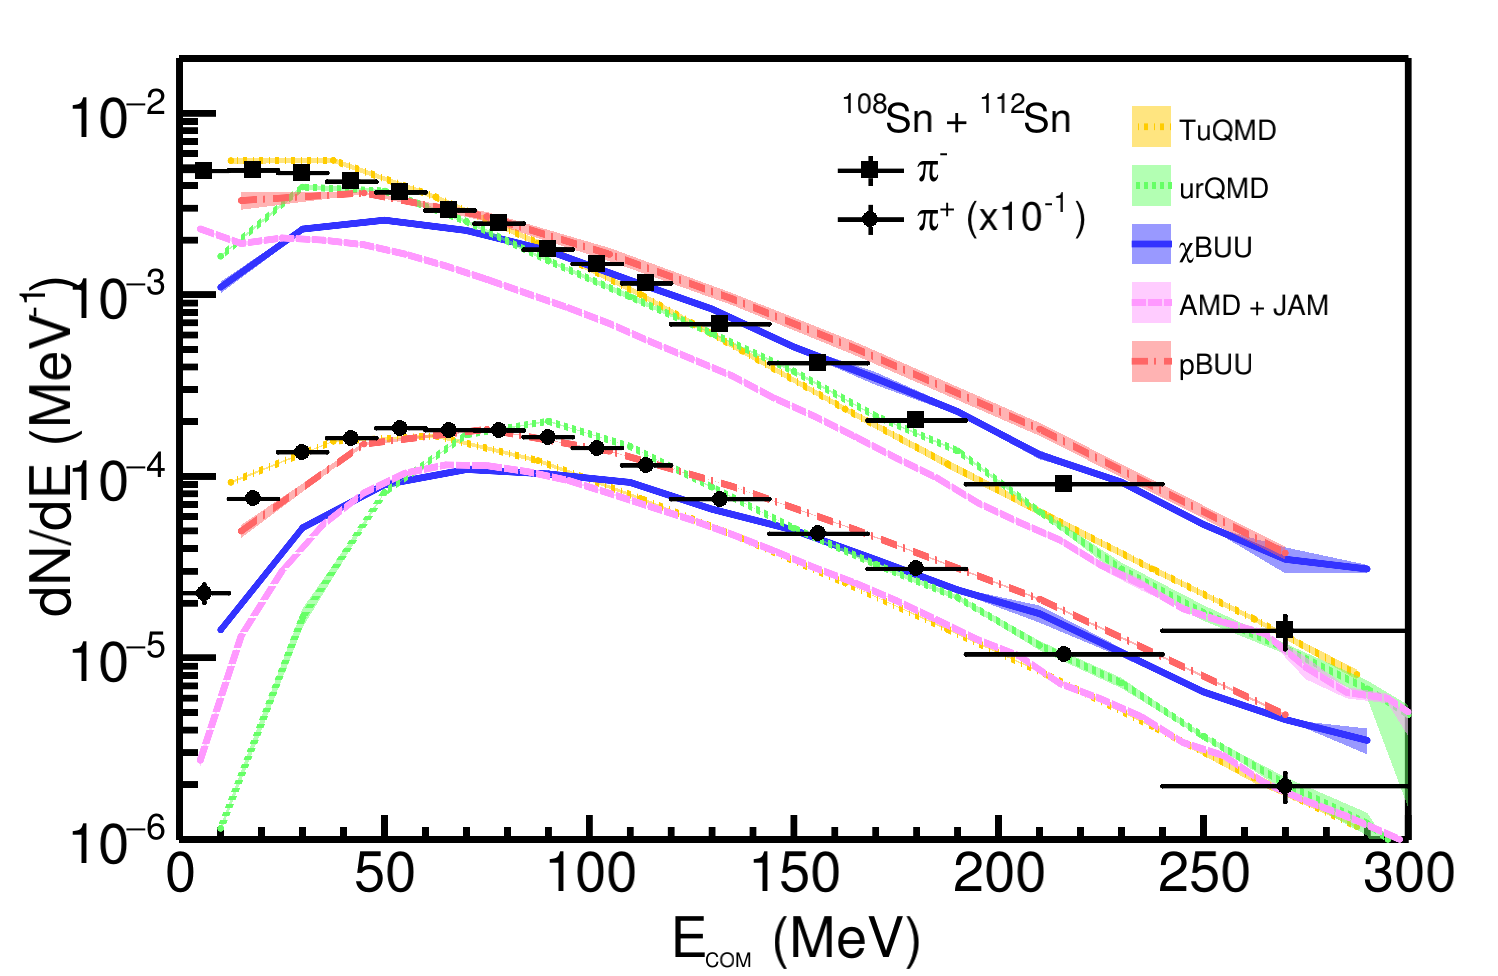
\includegraphics[width=\textwidth]{pionSpectra.png}
\caption{Pion spectra. }
\label{fig:pionspectra}
\end{figure}


%Add figure on Glauber model 
%Add figure on comparison to FOPI data

\section{Pion Yield}

The integrated pion yield for both systems and the $\pi^-/\pi^+$ ratio is listed in Table~\ref{tb:pionyield}, where the systematic errors are the first error bar and the statistical error is listed next. It is remarkable that the pion ratio is significantly greater than the N/Z of the system which is what is expected in the Delta Resonance model or under the assumption of chemical equilibrium which is $\pi^-/\pi^+ = (N/Z)^2$ CITE HERE; 2x in the $\tin{132}{124}$ system and 1.4x in the $\tin{108}{112}$ system. The pion ratio was hypothesized to be proportional to the high density N/Z ratio of the early system, where the other effects such as pion absorption and re-emission would dilute the effect and lower the ratio as the system tends toward isospin equilibrium. A na\"ive interpretation would be the high density N/Z fraction is much higher for some reason than the two systems, though, the system spends very little time in this state which would require a very soft Symmetry Energy. A more likely conclusion is the mechanisms involved in pion productions via the $\Delta(1232)$ resonance is more complicated than the simple $(N/Z)^2$ relation. For example the $\Delta$ resonance potential has an iso-scalar component (independent of iso-spin) and an iso-vector component. The nature of these two potentials is still unknown CITE HERE, and the role it plays in pion production has shown to be very important CITE HERE.


\begin{table*}\centering
\ra{1.3}
\begin{tabular}{@{}cccc@{}}\toprule
System & $\pi^-$ & $\pi^+$ & $Y(\pi^-)/Y(\pi^+)$  \\
\midrule
$\tin{132}{124}$ & 0.717(24)(4) & 0.148(5)(2) & 4.84(10)(6)  \\
$\tin{108}{112}$ & 0.399(14)(3) & 0.200(8)(2) & 1.99(4)(3)  \\
%$\tin{132}{124}$ & \numerr{0.717}{0.024}{0.004} & \numerr{0.148}{0.005}{0.002} & \numerr{4.84}{0.10}{0.06}  \\
%$\tin{108}{112}$ & \numerr{0.399}{0.014}{0.003} & \numerr{0.200}{0.008}{0.002} & \numerr{1.99}{0.04}{0.03}  \\
\bottomrule
\end{tabular}
\caption{Total pion yield.}
\label{tb:pionyield}
\end{table*}


We have compared the total pion yields and ratios to the 6 common transport codes for the systems measured. The table of the transport codes are listed in Appendix~\ref{tb:pionyieldTheory}. Figure~\ref{fig:totalpiYield} shows the total pion yield for the four systems measured as compared with the codes. The codes plotted here are only the soft symmetry energy since the variation in code is much larger than the intra-code variation between different Symmetry Energies. While some codes make a reasonable approximation of a particular charge pion, no code reasonably predict both. 

\begin{figure}[!htb]
\centering
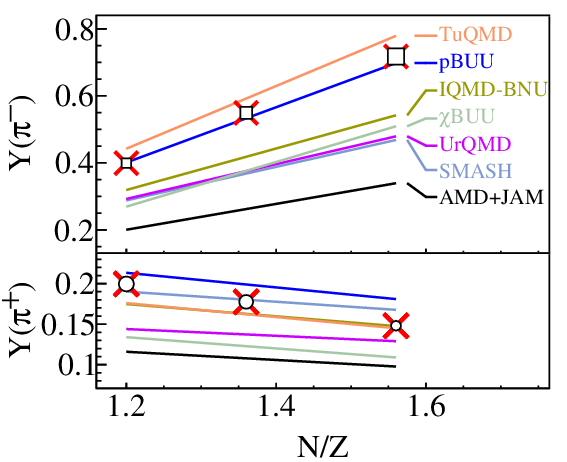
\includegraphics[width=.8\textwidth]{totalpiYield.png}
\caption{Total pion yields as compared with 6 common transport codes.}
\label{fig:totalpiYield}
\end{figure}

Figure~\ref{fig:totalpiRatio} shows the total single pion ratio and the double ratio of the $\tin{132}{124}$ and $\tin{108}{112}$ system. Here, the variation between codes is much larger than the variation between the Symmetry Energy within a particular code. The Symmetry Energy variation of two codes -- $\chi$BUU and TuQMD -- is plotted as a wide band in the single ratio and all codes in the double ratio; the data band represents the data error bar. Certainly the variation between Symmetry Energy in the $\tin{132}{124}$, though small, still exists in many of the codes as predicted initially CITE HERE BAO ANN. The small error bars in the data also would allow for a detailed analysis to extract a constraint of the Symmetry Energy, if the variation between codes could be solved. 



\begin{figure}[!htb]
\centering
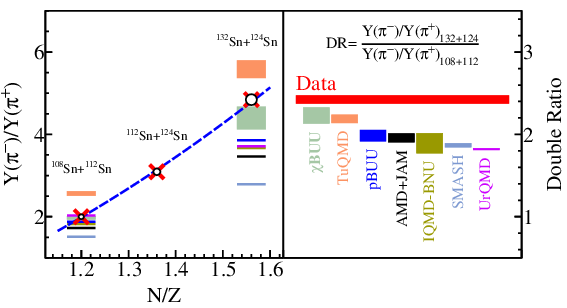
\includegraphics[width=\textwidth]{totalpiRatio.png}
\caption{Total pion ratio and double ratio compared with 6 common transport codes.}
\label{fig:totalpiRatio}
\end{figure}



\section{Pion Spectral Ratio}


\begin{figure}
\centering
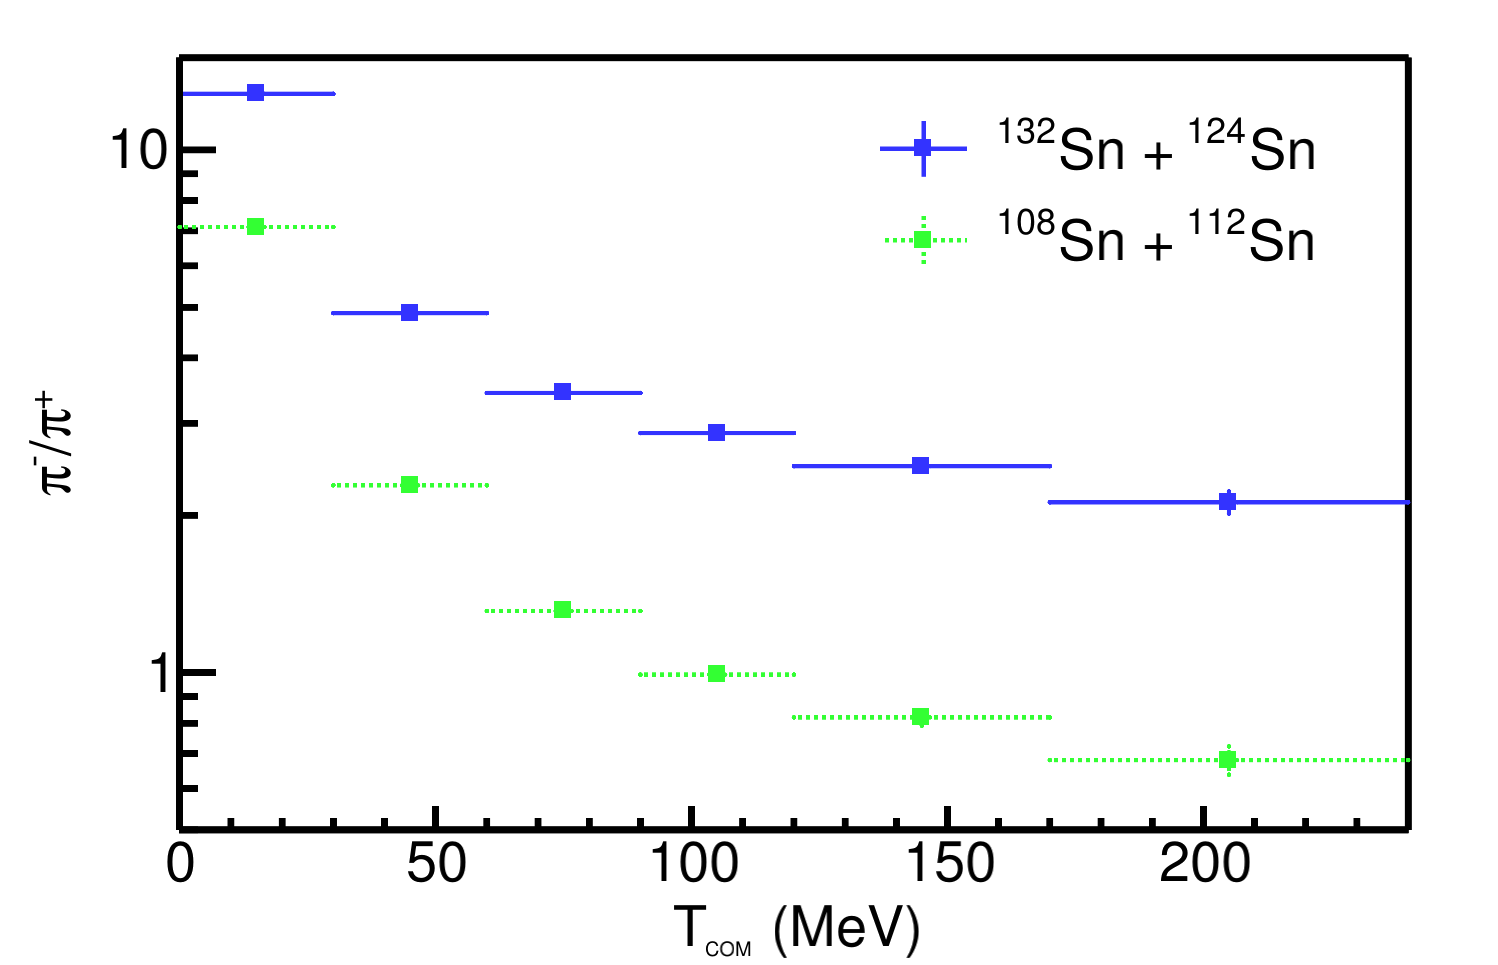
\includegraphics[width=\textwidth]{singleRatio.png}
\caption{Single ratio spectra}
\label{fig:SRspectra}
\end{figure}

%Add figure of Theory for pion ratios

\section{Pion Double Ratio}
%Add figure of Theory for pion ratios

\begin{figure}[!htb]
\centering
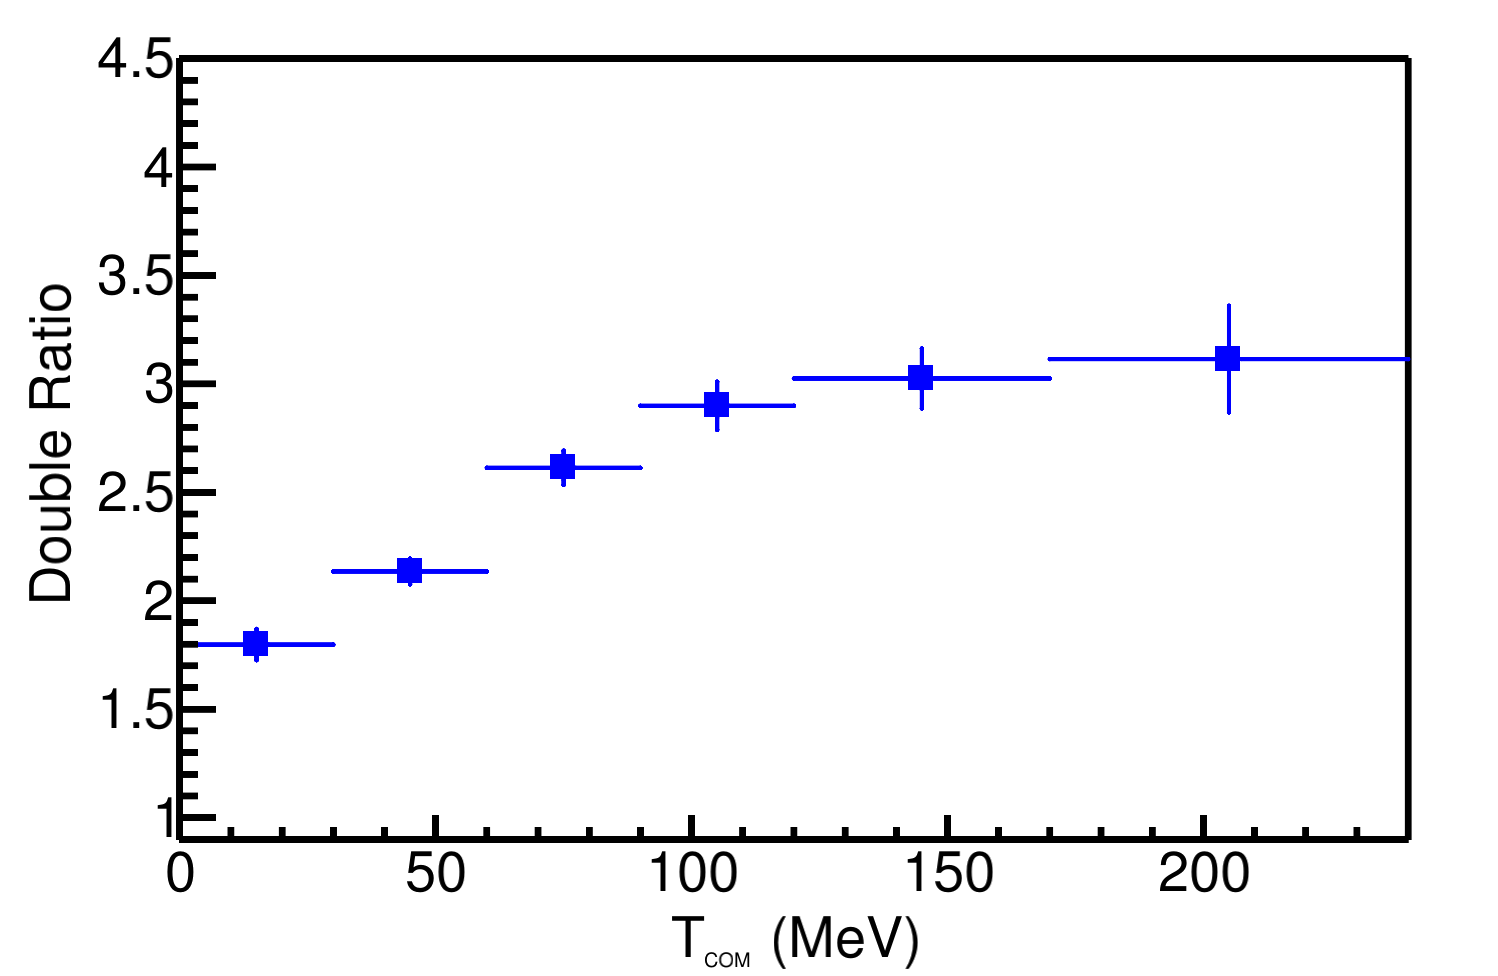
\includegraphics[width=\textwidth]{doubleRatio.png}
\caption{}
\label{fig:spectraDR}
\end{figure}




\section{Comparison to Previous Data Sets (FOPI)}
asdfasdfasd
\section{Comparison to Theory}
%Add figure of Pion spectra for different theory 
%Reference paper for multiple theories
asdfasdf

\section{Systematic Errors and Cut Variations}
\label{sec:cutvar}
dfsadfsaf
\section{Constraint on the Symmetry Energy}
%maybe not...